
\begin{frame}
\frametitle{Unsupervised Pretraining and Supervised Fine Tuning}

\begin{columns}
\column{.5\textwidth}
\textbf{GPT-2 Model}
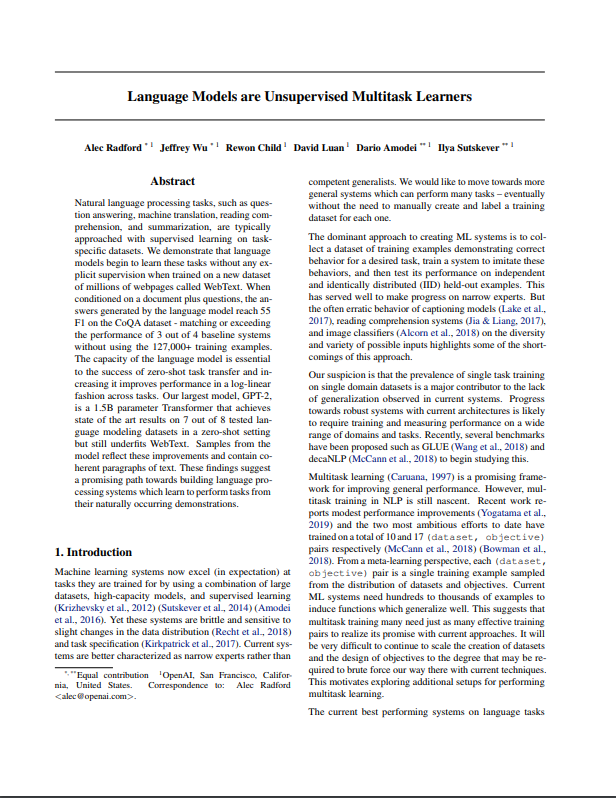
\includegraphics[width=2cm]{images/GPT2-paper}
{\small Radford, A., Wu, J., Child, R., Luan, D., Amodei, D., \& Sutskever, I. (2019). Language models are unsupervised multitask learners. URL https://openai. com/blog/better-language-models.}

\column{.5\textwidth}

\textbf{Bert Model}
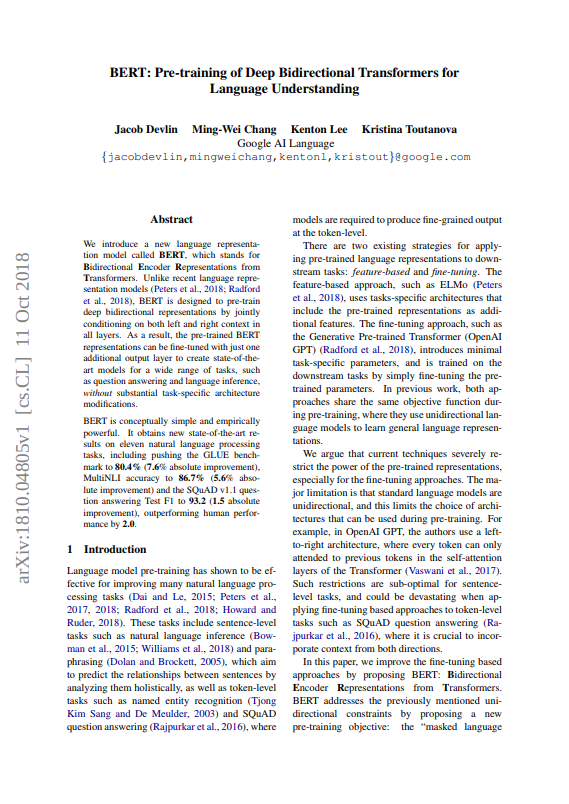
\includegraphics[width=2cm]{images/BERT-paper}

{\small Devlin, J., Chang, M. W., Lee, K., \& Toutanova, K. (2018). Bert: Pre-training of deep bidirectional transformers for language understanding. arXiv preprint arXiv:1810.04805.}

\end{columns}

\end{frame}

\begin{frame}
\frametitle{Unsupervised Clustering}

\begin{columns}
\column{.5\textwidth}
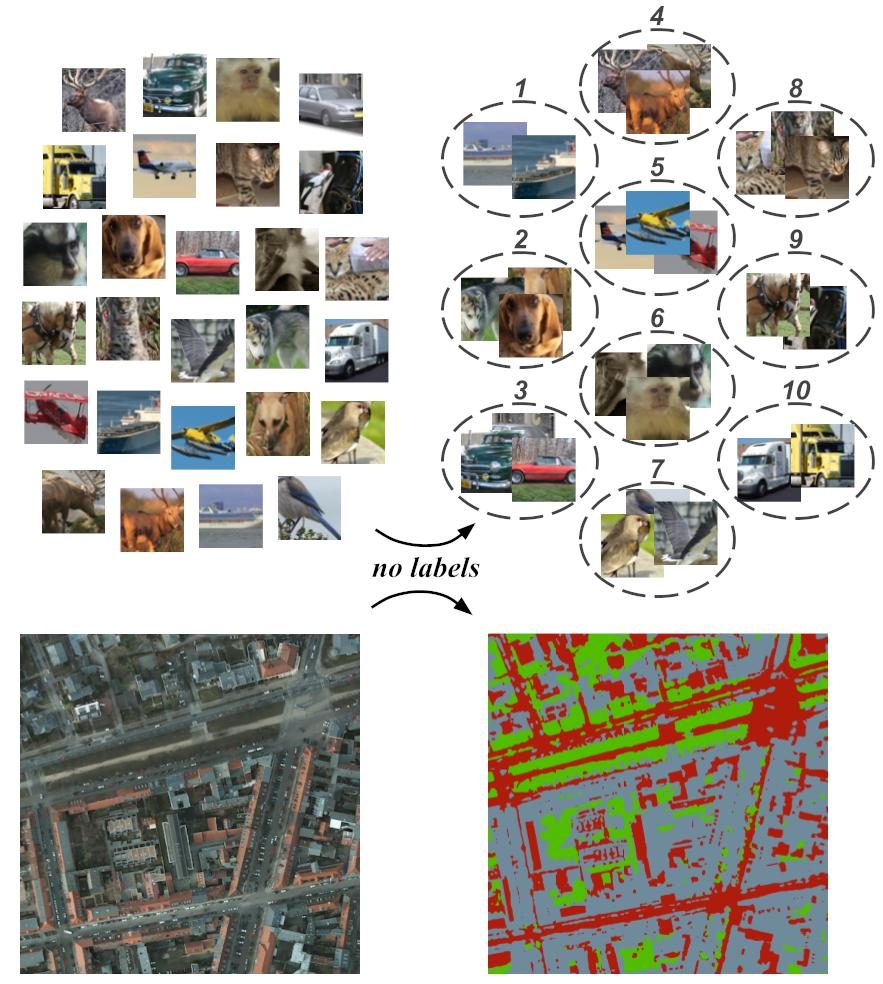
\includegraphics[width=.5\textwidth]{images/IIC_clustering}

{\small Xu Ji, Jo F. Henriques \& Andrea Vedaldi (2019). Invariant Information Distillation for Unsupervised Image Segmentation and Clustering. arXiv preprint arXiv:1807.06653}

\column{.5\textwidth}
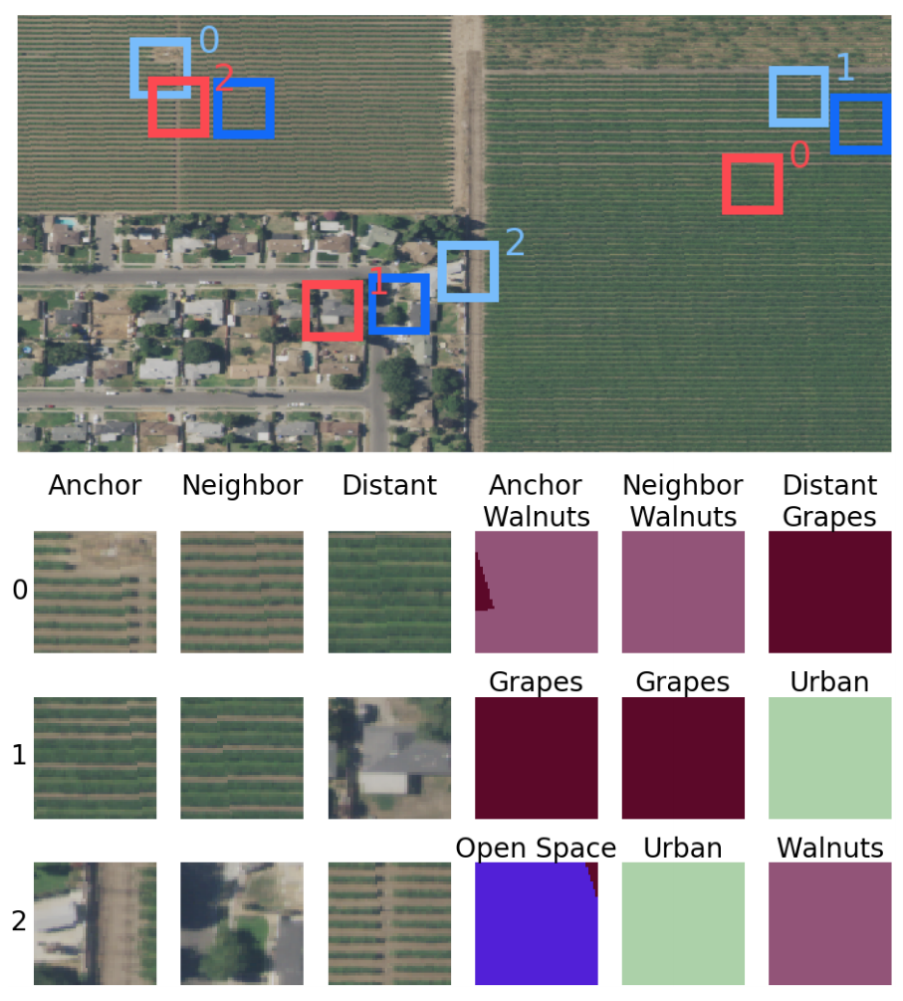
\includegraphics[width=.5\textwidth]{images/jean19_results}

{\small Jean, N., Wang, S., Azzari, G., Lobell, D., \& Ermon, S. (2018). Tile2Vec: Unsupervised representation learning for remote sensing data. arXiv preprint arXiv:1805.02855.}


\end{columns}


\end{frame}
%
%{\setbeamercolor{background canvas}{bg=tumblue}
%	\begin{frame}[plain]
%	\vfill
%	\begin{center}
%		\Huge\color{white}
%		Part III: Machine Learning + Earth Observation
%%		
\includegraphics[width=5cm]{images/TUM-white}
%	\end{center}
%	
%	\vfill
%\end{frame}
%}
%
%\begin{frame}
%	\frametitle{Crop Yield Prediction}
%		
%\end{frame}
%
%\begin{frame}
%	\frametitle{Alejandro Norega}
%		
%\end{frame}
%
%\begin{frame}
%	\frametitle{XX Zhu}
%
%\end{frame}